\chapter{The Interpreter}
\label{cha:Interpreter}

\section{Interpreter Overview}
\par \noindent The LUMEN interpreter is a programm that directly executes instructions from a LUMEN source file without previously compiling them into a machine language program. The LUMEN preprocessor first translate a LUMEN source file into an 
intermediate representation. This preprocessor consist out of three staps as shown in figure~\ref{fig:InterpreterWorking}. \bigskip

\par \noindent 

\begin{figure}[h]
    \centering
	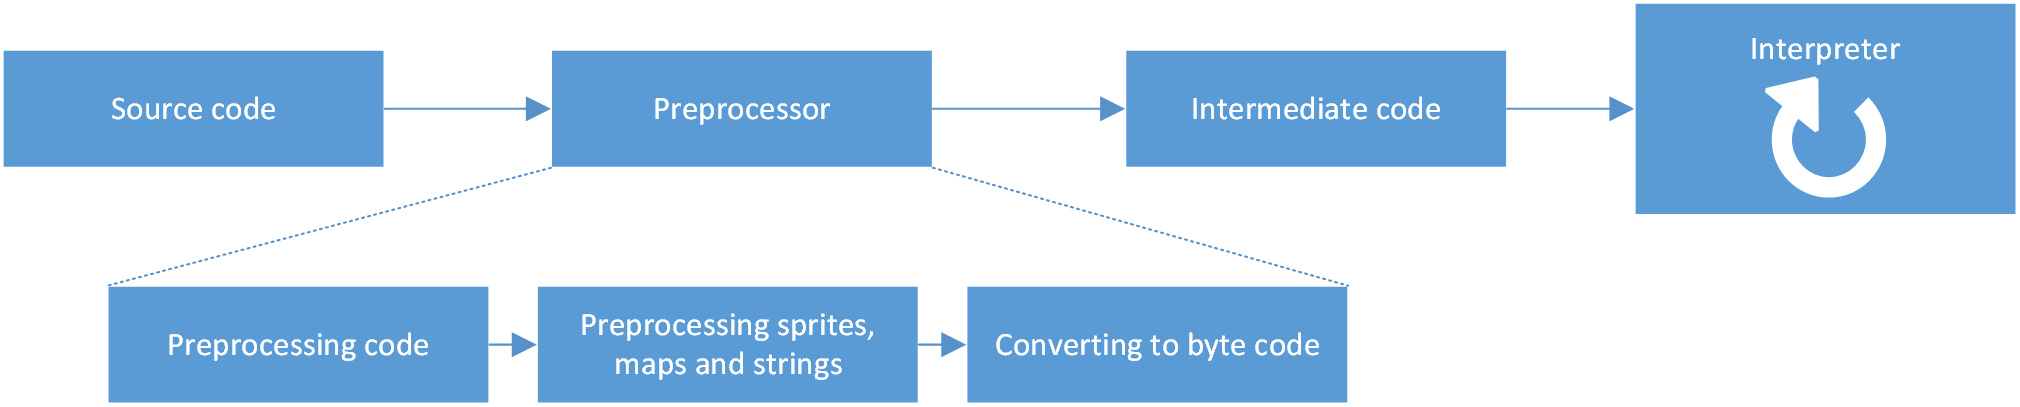
\includegraphics[width=13cm]{InterpreterWorking}
    \caption{LUMEN Interpreter chain}\par
    \label{fig:InterpreterWorking}
\end{figure}
